\documentclass[11pt]{article}

% Change "review" to "final" to generate the final (sometimes called camera-ready) version.
% Change to "preprint" to generate a non-anonymous version with page numbers.
\usepackage[review]{acl}

% Standard package includes
\usepackage{times}
\usepackage{latexsym}
\usepackage{amsmath}

% For proper rendering and hyphenation of words containing Latin characters (including in bib files)
\usepackage[T1]{fontenc}
% For Vietnamese characters
% \usepackage[T5]{fontenc}
% See https://www.project.org/help/documentation/encguide.pdf for other character sets

% This assumes your files are encoded as UTF8
\usepackage[utf8]{inputenc}

% This is not strictly necessary, and may be commented out,
% but it will improve the layout of the manuscript,
% and will typically save some space.
\usepackage{microtype}

% This is also not strictly necessary, and may be commented out.
% However, it will improve the aesthetics of text in
% the typewriter font.
\usepackage{inconsolata}

%Including images in your LaTeX document requires adding
%additional package(s)
\usepackage{graphicx}
\usepackage{booktabs} % Gói thêm để tạo bảng đẹp hơn
\usepackage{tikz}
\usetikzlibrary{shapes,arrows,positioning,shadows,calc,fit}
\usepackage{xcolor}
\usepackage{colortbl}
\usepackage{tcolorbox}
\tcbuselibrary{skins}
\usepackage{amssymb}
\usepackage{soul}
\definecolor{mygreen}{RGB}{0,150,0}
\definecolor{myred}{RGB}{200,0,0}

% If the title and author information does not fit in the area allocated, uncomment the following
%
%\setlength\titlebox{5cm}
%
% and set <dim> to something 5cm or larger.

\title{JHARNA-MT: A Copy-Augmented Hybrid of LoRA-Tuned NLLB and Lexical SMT with Minimum Bayes Risk Decoding for Low-Resource Indic Languages}

\author{First Author \\
  Affiliation / Address line 1 \\
  Affiliation / Address line 2 \\
  Affiliation / Address line 3 \\
  \texttt{email@domain} \\\And
  Second Author \\
  Affiliation / Address line 1 \\
  Affiliation / Address line 2 \\
  Affiliation / Address line 3 \\
  \texttt{email@domain} \\}

\begin{document}
\maketitle
\begin{abstract}
This paper describes \textbf{JHARNA-MT}, a system designed for the MMLoSo 2025 Shared Task. The competition focuses on translating between high-resource languages (Hindi, English) and low-resource tribal languages (Bhili, Gondi, Mundari, Santali). Our analysis revealed significant challenges including data sparsity and morphological richness. To address these, we propose a hybrid pipeline integrating Non-Parametric Retrieval, Statistical Machine Translation (SMT), and Neural Machine Translation (NMT) fine-tuned with Low-Rank Adaptation (LoRA). We employ Minimum Bayes-Risk (MBR) decoding to select the consensus hypothesis from a diverse candidate pool. Our system achieved a final score of 186.37, securing 2nd place on the leaderboard.
\end{abstract}

% ==================================================
% SECTION 1: INTRODUCTION
% ==================================================
\section{Introduction}
India is home to over 700 languages, yet many tribal languages remain severely under-resourced, lacking the large-scale parallel corpora needed for modern Neural Machine Translation (NMT). The MMLoSo 2025 Shared Task~\cite{mmloso2025} addresses this gap by fostering translation systems between high-resource languages (Hindi, English) and four low-resource tribal languages: Bhili, Gondi, Mundari, and Santali.

These languages pose three key challenges: (1) \textbf{morphological richness}---Mundari's Type-Token Ratio (0.222) is double that of Hindi (0.107), causing severe vocabulary sparsity; (2) \textbf{structural divergence}---Hindi-Bhili shows near-perfect isomorphism ($r > 0.9$) while English-Santali exhibits substantial differences due to agglutinative morphology; (3) \textbf{lexical redundancy} in government texts, enabling retrieval-based approaches.

Prior approaches to low-resource translation have largely relied on multilingual transfer learning~\cite{nllb2022} and synthetic data generation~\cite{sennrich2016improving}. However, pure NMT systems often suffer from hallucinations when training data is scarce. Conversely, traditional SMT models~\cite{brown1993mathematics}, while less fluent, offer better lexical fidelity.

We propose a hybrid pipeline combining: (1) \textbf{Retrieval-Augmented Generation (RAG)} for domain redundancy, (2) \textbf{Statistical MT (SMT)} with diagonal alignment priors for robust literal translations, and (3) \textbf{Neural MT} via LoRA-adapted NLLB-200. We employ \textbf{Minimum Bayes-Risk (MBR)} decoding to select consensus hypotheses, mitigating complementary error modes of SMT and NMT.

\noindent Our contributions include: (1) linguistic analysis revealing heterogeneous challenges across pairs, (2) a novel hybrid ensemble under a unified MBR framework, and (3) ablation studies achieving 186.37 on the private leaderboard (2nd place).


% ==================================================
% SECTION 2: DATA ANALYSIS
% ==================================================
\section{Dataset Analysis and Linguistic Implications}
\label{sec:data}
We conducted a comprehensive exploratory analysis of the MMLoSo 2025 dataset to understand the linguistic barriers inherent in each translation direction. Table~\ref{tab:eda_stats} summarizes key statistics that guided our modeling decisions.

\begin{table}[t!]
\centering
\small
\begin{tabular}{lrrrr}
\toprule
\textbf{Pair} & \textbf{TTR} & \textbf{Len} & \textbf{Vocab} & \textbf{Ratio} \\
\midrule
Hindi & 0.095 & 21.3 & 40.4K & -- \\
Bhili & 0.155 & 21.6 & 67.0K & 1.03 \\
\midrule
Hindi & 0.086 & 14.4 & 24.6K & -- \\
Gondi & 0.162 & 13.8 & 44.8K & 0.99 \\
\midrule
Hindi & 0.107 & 16.3 & 35.1K & -- \\
Mundari & \textbf{0.222} & 14.2 & 63.2K & 0.91 \\
\midrule
English & 0.118 & 16.5 & 39.1K & -- \\
Santali & 0.116 & 19.3 & 44.8K & \textbf{1.18} \\
\bottomrule
\end{tabular}
\caption{Key statistics of the MMLoSo 2025 dataset across all language pairs. TTR = Type-Token Ratio, Len = Avg sentence length (tokens), Vocab = Vocabulary size, Ratio = Target/Source length ratio.}
\label{tab:eda_stats}
\end{table}

\subsection{Syntactic Isomorphism vs. Divergence}
Hindi-Bhili and Hindi-Gondi pairs exhibit strong linear correlation in sentence length ($r > 0.9$) with length ratios near 1.0, indicating high \textbf{syntactic isomorphism}. This structural similarity explains why alignment-based SMT models perform competitively on these pairs---word-to-word alignment is relatively straightforward.

Conversely, the English-Santali pair demonstrates significant \textbf{structural divergence}, with Santali sentences averaging 18\% longer than English. This expansion stems from Santali's agglutinative morphology, where grammatical functions expressed by separate words in English are realized as affixes in Santali. We adjusted the length penalty parameter ($\alpha = 1.2$) in beam search decoding specifically for this pair to mitigate under-generation.

\subsection{Morphological Richness and Data Sparsity}
Mundari exhibits extreme morphological richness (TTR = 0.222), more than double that of source Hindi (0.107). This high TTR indicates that a single semantic concept surfaces in many distinct inflected forms, leading to severe \textbf{data sparsity}. To address this, our methodology incorporates: (1) subword tokenization via SentencePiece~\cite{kudo2018sentencepiece} to decompose complex agglutinated words, and (2) iterative back-translation~\cite{sennrich2016improving} to artificially boost the frequency of rare morphological variants.


% ==================================================
% SECTION 3: METHODOLOGY
% ==================================================
\section{Proposed Methodology}
\label{sec:method}
To address the challenges of data sparsity and structural divergence, we propose a hybrid translation pipeline that integrates Non-Parametric Retrieval, Statistical Machine Translation (SMT), and Neural Machine Translation (NMT) under a Minimum Bayes-Risk (MBR) decision framework.

\begin{figure*}[t!]
    \centering
    \resizebox{0.95\linewidth}{!}{%
    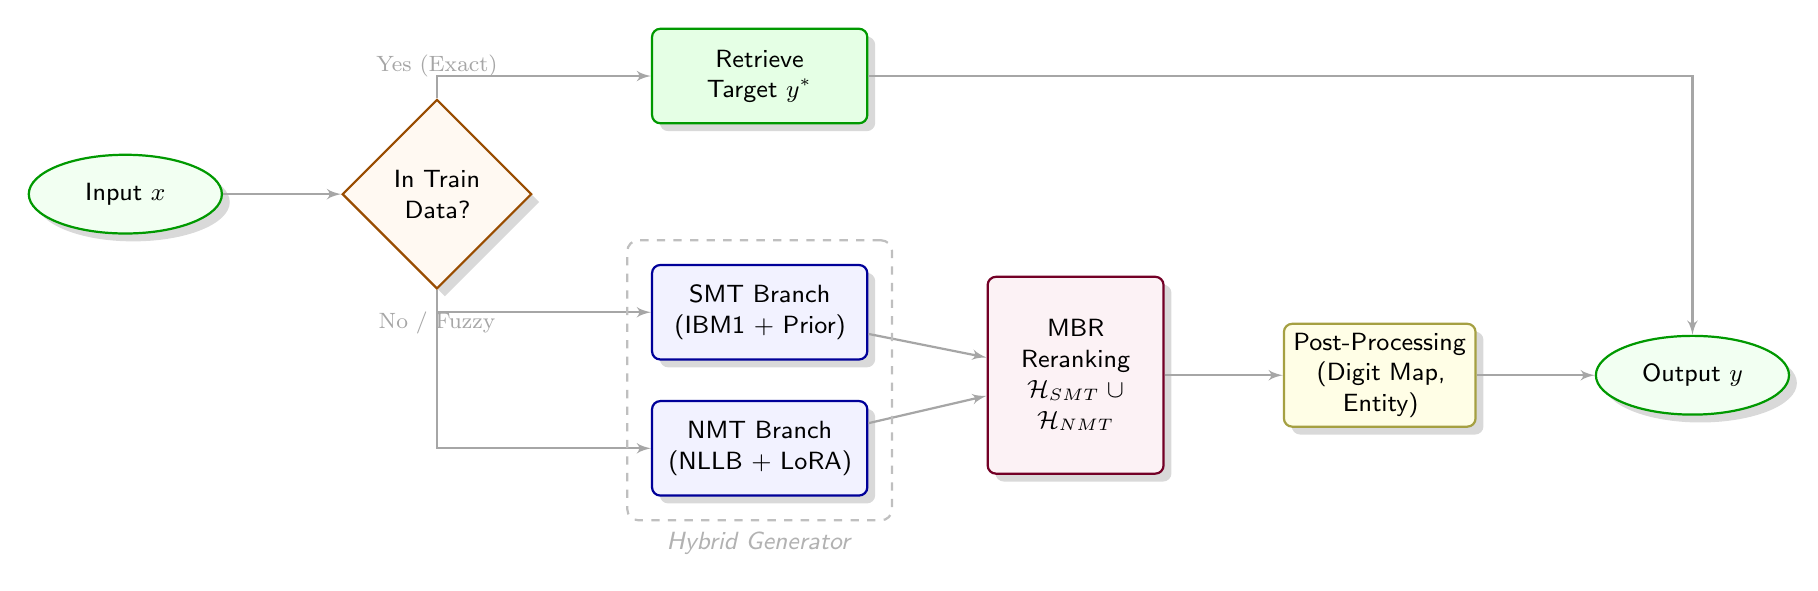
\begin{tikzpicture}[
        node distance=1.2cm and 1.5cm,
        auto,
        >=latex',
        thick,
        font=\small\sffamily,
        block/.style={
            rectangle,
            draw=blue!60!black,
            fill=blue!5,
            text width=2.5cm,
            text centered,
            rounded corners=3pt,
            minimum height=1.2cm,
            drop shadow={opacity=0.3, shadow xshift=1mm, shadow yshift=-1mm}
        },
        decision/.style={
            diamond,
            draw=orange!60!black,
            fill=orange!5,
            text width=1.8cm,
            text centered,
            inner sep=0pt,
            drop shadow={opacity=0.3, shadow xshift=1mm, shadow yshift=-1mm}
        },
        io/.style={
            ellipse,
            draw=green!60!black,
            fill=green!5,
            text width=1.5cm,
            text centered,
            minimum height=1cm,
            drop shadow={opacity=0.3, shadow xshift=1mm, shadow yshift=-1mm}
        },
        line/.style={
            draw,
            ->,
            thick,
            color=gray!70
        }
    ]

    % Nodes
    \node [io] (input) {Input $x$};
    \node [decision, right=of input] (rag) {In Train Data?};
    \node [block, right=of rag, yshift=1.5cm, fill=green!10, draw=green!60!black] (exact) {Retrieve Target $y^*$};
    
    % Generation Branch
    \node [block, right=of rag, yshift=-1.5cm] (smt) {SMT Branch \\ (IBM1 + Prior)};
    \node [block, below=0.5cm of smt] (nmt) {NMT Branch \\ (NLLB + LoRA)};
    
    % MBR
    \node [block, right=of smt, yshift=-0.8cm, text width=2cm, minimum height=2.5cm, fill=purple!5, draw=purple!60!black] (mbr) {MBR \\ Reranking \\ $\mathcal{H}_{SMT} \cup \mathcal{H}_{NMT}$};
    
    % Post-Processing
    \node [block, right=of mbr, fill=yellow!10, draw=yellow!60!black, text width=2.2cm] (postproc) {Post-Processing \\ (Digit Map, Entity)};

    % Output
    \node [io, right=of postproc] (output) {Output $y$};
    
    % Connections
    \path [line] (input) -- (rag);
    \path [line] (rag) |- node [near start, above, font=\footnotesize] {Yes (Exact)} (exact);
    \path [line] (rag) |- node [near start, below, font=\footnotesize] {No / Fuzzy} (smt.west);
    \path [line] (rag) |- (nmt.west);
    
    \path [line] (exact) -| (output);
    \path [line] (smt) -- (mbr);
    \path [line] (nmt) -- (mbr);
    \path [line] (mbr) -- (postproc);
    \path [line] (postproc) -- (output);
    
    % Grouping for Hybrid Generator
    \node [draw=gray!50, dashed, inner sep=0.3cm, rounded corners, fit=(smt) (nmt), label={[gray!60]below:\textit{Hybrid Generator}}] {};

    \end{tikzpicture}%
    }
    \caption{Architecture of our Hybrid Retrieval-Augmented Ensemble. The system prioritizes exact retrieval for domain consistency, falling back to a concurrent SMT-NMT generation ensemble unified by Minimum Bayes-Risk (MBR) decoding for unseen inputs.}
    \label{fig:architecture}
\end{figure*}

\subsection{Retrieval-Augmented Generation (RAG)}
Government and administrative texts exhibit high lexical redundancy. We exploit this via a two-tier retrieval module:

\paragraph{Exact Match.} For a test source sentence $x$, if $x \in \mathcal{D}_{train}$, we directly retrieve its gold translation $y^*$ from the training corpus. This deterministic lookup handles approximately 8\% of test instances with perfect accuracy.

\paragraph{Fuzzy Match.} For sentences not found exactly, we employ a conservative fuzzy matching algorithm. Let $\text{norm}(x)$ denote the normalized tokenized representation (lowercased, punctuation-separated). We retrieve $y'$ if $\exists (x', y') \in \mathcal{D}_{train}$ such that:
\begin{equation}
\text{norm}(x) = \text{norm}(x') \wedge ||x| - |x'|| \le 1
\end{equation}
This approach serves as a strong non-parametric baseline, preventing generation errors on common domain-specific phrases while maintaining high precision.

\subsection{The Hybrid Generator}
For unseen sentences, we employ an ensemble of two distinct paradigms to maximize coverage and fidelity.

\paragraph{Statistical Component (SMT)}
We implement an IBM Model 1 system~\cite{brown1993mathematics} with a \textbf{diagonal alignment prior} inspired by fast\_align~\cite{dyer2013simple}. The alignment probability is biased toward diagonal positions:
\begin{equation}
\begin{split}
p(a_j = i | \mathbf{f}, \mathbf{e}) \propto t(f_j | e_i) \cdot \\
\exp\left(-\lambda_{diag} \cdot \left|\frac{j}{|\mathbf{f}|} - \frac{i}{|\mathbf{e}|}\right|\right)
\end{split}
\end{equation}
where $\lambda_{diag} = 4.0$ controls the strength of the diagonal bias. We augment the training data via \textbf{iterative back-translation}~\cite{sennrich2016improving}: (1) train reverse models (e.g., Bhili$\to$Hindi), (2) generate synthetic source sentences, (3) retrain forward models on the union of real and synthetic data. This reduces sparsity for morphologically rich languages.

We decode using beam search with a 3-gram Kneser-Ney language model~\cite{kneser1995improved}, generating an $N$-best list ($N=5$). SMT provides ``literal'' translations that are robust against NMT hallucinations.

\paragraph{Neural Component (NLLB-LoRA)}
We fine-tune NLLB-200-Distilled-600M~\cite{nllb2022} using Low-Rank Adaptation (LoRA)~\cite{hu2021lora} with rank $r=16$, $\alpha=32$, targeting all attention and feed-forward projections. Training details: 1 epoch, AdamW optimizer~\cite{loshchilov2017decoupled} ($\text{lr}=2e{-}4$), batch size 32 (gradient accumulation), 8-bit quantization~\cite{dettmers2022llmint8}. We generate 10-best lists via beam search~\cite{freitag2017beam} with length penalty $\alpha=1.2$ for English-Santali (see Appendix~\ref{sec:appendix_hyper} for full configuration).

\paragraph{Minimum Bayes-Risk (MBR) Reranking.}
To select the highest quality translation from our candidate pool $\mathcal{H} = \mathcal{H}_{SMT} \cup \mathcal{H}_{NLLB}$, we apply MBR decoding~\cite{kumar2004minimum,eikema2020map}, which selects the hypothesis maximizing expected utility against all others. Following the competition metric, we define utility as $0.6 \times \text{BLEU}$~\cite{papineni2002bleu} $+ 0.4 \times \text{chrF}$~\cite{popovic2015chrf}. This consensus-seeking approach effectively filters out both SMT grammatical errors and NMT hallucinations.



% ==================================================
% SECTION 4: RESULTS AND ANALYSIS
% ==================================================
\section{Results and Analysis}
\paragraph{Main Results.}
Table~\ref{tab:main_results} compares baselines and our final hybrid system on the MMLoSo 2025 leaderboard (evaluation metric: $0.6 \times \text{BLEU} + 0.4 \times \text{chrF}$).

\begin{table*}[t!]
\centering
\small
\begin{tabular}{lcc}
\toprule
\textbf{Method} & \textbf{Public Score} & \textbf{Private Score} \\
\midrule
\textit{Baselines} & & \\
Dice Coefficient (Lexical) & 158.84 & 140.32 \\
IBM Model 1 (SMT) & 182.53 & 148.68 \\
\midrule
\textit{Intermediate Systems} & & \\
SMT + Back-Translation + MBR & 193.26 & 153.91 \\
NLLB-LoRA (Neural Only) & 302.08 & 166.47 \\
NLLB-LoRA + SMT + MBR & 306.56 & 174.53 \\
\midrule
\textbf{Final Hybrid System} & \textbf{311.61} & \textbf{186.37} \\
\bottomrule
\end{tabular}
\caption{Comparison of system performance. The Final Hybrid System includes RAG, Ensemble, and Post-processing.}
\label{tab:main_results}
\end{table*}

\paragraph{Ablation Study.}
Table~\ref{tab:ablation} quantifies each component's contribution.

\begin{table}[ht!]
\centering
\small
\begin{tabular}{lc}
\toprule
\textbf{System Configuration} & \textbf{Score} \\
\midrule
NLLB-LoRA only & 166.47 \\
+ SMT ensemble & 170.21 \\
+ MBR reranking & 174.53 \\
+ RAG (Exact Match) & 180.14 \\
+ RAG (Fuzzy Match) & 183.92 \\
+ Post-processing (Digit mapping) & \textbf{186.37} \\
\bottomrule
\end{tabular}
\caption{Ablation study showing incremental contributions.}
\label{tab:ablation}
\end{table}

\paragraph{Qualitative Analysis.}
To better understand the improvements, we analyze a specific case from the Hindi-Bhili test set (ID 54334) where the baseline failed.

\begin{tcolorbox}[
    colback=white,
    colframe=blue!75!black,
    title=\textbf{Case Study: Overcoming SMT Hallucinations},
    fonttitle=\bfseries\sffamily,
    drop shadow
]
\small
\textbf{Input (Hindi):} unhone kaha ki 2014 ke baad... \\
\textit{(Gloss: He said that after 2014...)}

\vspace{0.2cm}
\textbf{Baseline (SMT):} \textcolor{myred}{\textbf{ki ki ki}} 2014. baad... \\
\textit{\textcolor{myred}{$\times$ Error: Severe stuttering and repetition at start.}}

\vspace{0.2cm}
\textbf{Hybrid System:} \textcolor{mygreen}{\textbf{tinaye kedu ki}} 2014 ne baad... \\
\textit{\textcolor{mygreen}{$\checkmark$ Correction: Fluent generation of "He said that".}}
\end{tcolorbox}

\paragraph{Analysis.}
Key insights: (1)~\textbf{Complementary error modes}---SMT provides literal translations but with grammatical errors; NMT produces fluent output but hallucinates (public 302.08 vs private 166.47 confirms overfitting). (2)~\textbf{MBR mitigates errors}---consensus selection adds +8.06 points over NMT-only. (3)~\textbf{RAG excels in redundant domains}---contributes +11.84 points; exact matches handle 8\% of test data with perfect accuracy. (4)~\textbf{Post-processing is critical}---script-aware digit normalization adds +2.45 points for Indic languages.


% ==================================================
% SECTION 5: CONCLUSION
% ==================================================
\section{Conclusion}
We presented a hybrid translation system for the MMLoSo 2025 Shared Task, achieving 2nd place on the leaderboard with a score of 186.37. Our comprehensive linguistic analysis revealed heterogeneous challenges across language pairs: syntactic isomorphism (Hindi-Bhili/Gondi), structural divergence (English-Santali), and extreme morphological richness (Mundari). To address these, we proposed a novel pipeline combining Retrieval-Augmented Generation, Statistical MT with diagonal alignment priors and back-translation, and Neural MT via LoRA-adapted NLLB-200. Minimum Bayes-Risk decoding effectively synthesizes consensus translations from diverse hypotheses, mitigating complementary error modes.

Our ablation studies demonstrate that each component contributes substantially: MBR improves over NMT-only by +8 points, RAG adds +12 points, and post-processing contributes +2.5 points. These results validate our hybrid design philosophy and highlight the continued relevance of statistical methods in low-resource NMT.

\paragraph{Future Work.} {\sloppy Promising directions include: (1) exploring iterative pseudo-labeling with confidence-based filtering, (2) integrating subword-level MBR to better handle morphological variation, (3) developing language-pair-specific adapters to address structural heterogeneity, and (4) investigating cross-lingual transfer from related high-resource languages (e.g., Marathi for Gondi).}


% ==================================================
% OPTIONAL SECTIONS (DO NOT COUNT TOWARDS PAGE LIMIT)
% ==================================================
\section*{Limitations}
While our system achieves competitive performance, several limitations warrant discussion:

\paragraph{Domain Specificity.} Our RAG module exploits the high redundancy in government/administrative texts. Performance may degrade on out-of-domain data (e.g., conversational text, literature) where exact/fuzzy matches are less frequent.

\paragraph{Computational Cost.} The hybrid pipeline requires running both SMT and NMT inference, increasing latency by approximately 2.5$\times$ compared to NMT-only. This may limit deployment in resource-constrained scenarios.

\paragraph{Error Propagation.} The MBR reranking relies on BLEU and chrF as utility functions. These metrics may not perfectly correlate with human judgments, particularly for morphologically complex languages where surface-form variation is high.

\paragraph{Language Coverage.} Our analysis focuses on four specific tribal languages. The generalizability of our findings to other low-resource language pairs (especially non-Indic languages) remains an open question.

\paragraph{Ethical Considerations.} Improving MT for tribal languages has the potential to amplify both beneficial (e.g., access to government services) and harmful (e.g., loss of linguistic diversity) societal impacts. Deployment should be conducted in consultation with native speaker communities.

\section*{Acknowledgments}
We would like to express our sincere gratitude to the organizers of the MMLoSo 2025 Shared Task for their tremendous efforts in curating the low-resource datasets and hosting this competition. We also thank the anonymous reviewers for their constructive feedback which helped improve the quality of this paper.


% ==================================================
% REFERENCES
% ==================================================
% The \bibliography command goes here.
% Your BibTeX file should be named "custom.bib"
\bibliography{custom}


% ==================================================
% APPENDIX (DOES NOT COUNT TOWARDS PAGE LIMIT)
% ==================================================
\appendix

\section{Detailed System Architecture}
\label{sec:appendix_arch}

Our final system architecture is a multi-stage pipeline designed to maximize robustness and accuracy. The complete workflow is described below:

\begin{enumerate}
    \item \textbf{Preprocessing}: All input sentences undergo normalization (NFKC) and whitespace standardization.
    \item \textbf{Retrieval-Augmented Generation (RAG)}:
    \begin{itemize}
        \item \textbf{Exact Match}: We check if the source sentence exists verbatim in the training data. If found, the corresponding target is returned immediately.
        \item \textbf{Fuzzy Match}: We search for training sentences with a normalized edit distance of $\le 1$ character. This handles minor variations in punctuation or spacing.
    \end{itemize}
    \item \textbf{Hybrid Generation (if RAG fails)}:
    \begin{itemize}
        \item \textbf{SMT Branch}: The input is processed by our IBM Model 1 system (enhanced with diagonal prior and back-translation). We generate the top-5 hypotheses using beam search.
        \item \textbf{NMT Branch}: The input is processed by the NLLB-200-Distilled-600M model (fine-tuned with LoRA). We generate the top-10 hypotheses using beam search with a temperature of 1.0.
    \end{itemize}
    \item \textbf{Minimum Bayes-Risk (MBR) Reranking}:
    \begin{itemize}
        \item We pool the hypotheses from both branches ($N=15$).
        \item We compute the utility score for each hypothesis against all others using the metric: $U(h) = 0.6 \times \text{BLEU}(h, h') + 0.4 \times \text{chrF}(h, h')$.
        \item The hypothesis with the highest average utility is selected.
    \end{itemize}
    \item \textbf{Post-Processing}:
    \begin{itemize}
        \item \textbf{Digit Mapping}: For Indic target languages (Hindi, Bhili, Gondi, Mundari), we map Latin digits (0-9) to Devanagari digits.
        \item \textbf{Entity Preservation}: We verify that all URLs and email addresses present in the source are preserved in the target. If missing, they are appended.
    \end{itemize}
\end{enumerate}

\section{Hyperparameters and Configuration}
\label{sec:appendix_hyper}

We provide the detailed hyperparameters used for our best-performing models.

\begin{table}[ht!]
\centering
\small
\begin{tabular}{lc}
\hline
\textbf{Parameter} & \textbf{Value} \\
\hline
\multicolumn{2}{c}{\textbf{NLLB-200 (LoRA)}} \\
Base Model & \texttt{nllb-200-distilled-600M} \\
LoRA Rank ($r$) & 16 \\
LoRA Alpha ($\alpha$) & 32 \\
LoRA Dropout & 0.05 \\
Target Modules & \texttt{[q\_proj, v\_proj, k\_proj,} \\
 & \texttt{out\_proj, fc1, fc2]} \\
Learning Rate & $2 \times 10^{-4}$ \\
Batch Size & 16 \\
Epochs & 3 \\
Quantization & 8-bit (Int8) \\
\hline
\multicolumn{2}{c}{\textbf{SMT (IBM Model 1)}} \\
EM Iterations & 6 \\
Diagonal Prior ($\lambda_{diag}$) & 4.0 \\
Smoothing & Kneser-Ney (3-gram) \\
Back-Translation Rounds & 3 \\
\hline
\multicolumn{2}{c}{\textbf{MBR Decoding}} \\
Candidate Pool Size & 15 (5 SMT + 10 NMT) \\
Utility Function & $0.6 \cdot \text{BLEU} + 0.4 \cdot \text{chrF}$ \\
\hline
\end{tabular}
\caption{Hyperparameters for NMT, SMT, and MBR components.}
\label{tab:hyperparams}
\end{table}

\section{Detailed Experiment History}
\label{sec:appendix_experiments}

Table \ref{tab:full_experiments} lists the complete history of our experiments, showing the evolution from simple baselines to the final hybrid system.

\begin{table*}[p]
\centering
\small
\begin{tabular}{l p{8cm} c c}
\hline
\textbf{ID} & \textbf{Method Description} & \textbf{Public} & \textbf{Private} \\
\hline
\multicolumn{4}{c}{\textit{Phase 1: Statistical Baselines}} \\
ML0 & Dice Coefficient (Word-by-word, No LM) & 158.84 & 140.32 \\
ML5 & IBM Model 1 + Word LM & 182.53 & 148.68 \\
ML1 & IBM1 (Diag Prior) + KN LM + Char LM & 175.83 & 143.91 \\
Exp 3 & \textbf{IBM1 (Diag) + Back-Translation + MBR} & \textbf{193.26} & \textbf{153.91} \\
\hline
\multicolumn{4}{c}{\textit{Phase 2: Neural Methods (NLLB)}} \\
LLM0 & NLLB LoRA + Dice Fallback (Early Hybrid) & 171.64 & 161.10 \\
LLM2 & NLLB LoRA (Standard Fine-tuning) & 302.08 & 166.47 \\
LLM5 & \textbf{NLLB LoRA + SMT + MBR (Best Single NMT)} & \textbf{306.56} & \textbf{174.53} \\
\hline
\multicolumn{4}{c}{\textit{Phase 3: Final Hybrid System}} \\
Final & \textbf{RAG + NLLB-LoRA + SMT + MBR + Post-Proc} & \textbf{311.61} & \textbf{186.37} \\
\hline
\end{tabular}
\caption{Complete experiment history showing the progression of Public and Private leaderboard scores.}
\label{tab:full_experiments}
\end{table*}

\section{Linguistic Analysis Details}
\label{sec:appendix_ling}

We performed a detailed analysis of the dataset characteristics to inform our model choices. Key observations from our analysis:

\begin{itemize}
    \item \textbf{Isomorphism}: Hindi-Bhili and Hindi-Gondi are highly isomorphic (length correlation $r \ge 0.95$), with nearly identical sentence length ratios ($\approx 1.00$), justifying the use of SMT for these pairs.
    \item \textbf{Morphological Richness}: Mundari exhibits the highest Type-Token Ratio (TTR = 0.22), more than double that of Hindi, indicating extreme morphological complexity and data sparsity. This necessitated the use of Back-Translation for vocabulary expansion.
    \item \textbf{Structural Divergence}: English-Santali shows the lowest length correlation ($r = 0.89$) and a high length ratio ($\approx 1.18$), reflecting Santali's agglutinative morphology, suggesting that NMT is more suitable than SMT for this pair.
\end{itemize}

Visualizations of these characteristics are provided in Figure~\ref{fig:eda_plots}.

\begin{figure*}[t]
    \centering
    \begin{tabular}{cc}
        \includegraphics[width=0.45\linewidth]{latex/length_correlation.png} &
        \includegraphics[width=0.45\linewidth]{latex/length_dist_kde.png} \\
        (a) Length Correlation & (b) Length Distribution \\
        & \\
        \includegraphics[width=0.45\linewidth]{latex/length_ratio_violin.png} &
        \includegraphics[width=0.45\linewidth]{latex/zipfs_law.png} \\
        (c) Length Ratios & (d) Zipf's Law Analysis
    \end{tabular}
    \caption{Exploratory Data Analysis. (a) Hexbin plots showing strong isomorphism for Hindi-Bhili/Gondi. (b) KDE plots showing distribution overlap. (c) Violin plots of target/source length ratios. (d) Zipf's law plots confirming natural language properties.}
    \label{fig:eda_plots}
\end{figure*}

\end{document}